\RequirePackage{plautopatch}
\documentclass[14pt,aspectratio=169,xcolor=dvipsnames,table,dvipdfmx]{beamer}
\usepackage{bxdpx-beamer} % dvipdfmxなので必要

%Beamerの設定
\usetheme{Boadilla}

%Beamerフォント設定
\usefonttheme{professionalfonts} % Be professional!
\usepackage[T1]{fontenc}
\usepackage{mlmodern}  % 太いComputer Modern
% MLmodernのバグを修正: cf. https://tex.stackexchange.com/questions/646333/size-of-integral-symbol-in-section-header-with-mlmodern
\DeclareFontFamily{OMX}{mlmex}{}
\DeclareFontShape{OMX}{mlmex}{m}{n}{%
   <->mlmex10%
   }{} 
\usepackage{newtxtext} % 数式以外をTXフォントで上書き
\usepackage[deluxe,uplatex]{otf} % 日本語多ウェイト化
\usepackage{physics,bm}
\usepackage{mhchem}
\usepackage{amsmath,amsfonts,amssymb,mathtools,amsthm}
\renewcommand{\familydefault}{\sfdefault}  % 英文をサンセリフ体に
\renewcommand{\kanjifamilydefault}{\gtdefault}  % 日本語をゴシック体に
\usefonttheme{structurebold} % タイトル部を太字
\setbeamerfont{alerted text}{series=\bfseries} % Alertを太字
\setbeamerfont{section in toc}{series=\mdseries} % 目次は太字にしない
\setbeamerfont{frametitle}{size=\Large} % フレームタイトル文字サイズ
\setbeamerfont{title}{size=\LARGE} % タイトル文字サイズ
\setbeamerfont{date}{size=\small}  % 日付文字サイズ

% Babel (日本語の場合のみ・英語の場合は不要)
\uselanguage{japanese}
\languagepath{japanese}
\deftranslation[to=japanese]{Theorem}{定理}
\deftranslation[to=japanese]{Lemma}{補題}
\deftranslation[to=japanese]{Example}{例}
\deftranslation[to=japanese]{Examples}{例}
\deftranslation[to=japanese]{Definition}{定義}
\deftranslation[to=japanese]{Definitions}{定義}
\deftranslation[to=japanese]{Problem}{問題}
\deftranslation[to=japanese]{Solution}{解}
\deftranslation[to=japanese]{Fact}{事実}
\deftranslation[to=japanese]{Proof}{証明}
\def\proofname{証明}

%Beamer色設定
\definecolor{UniBlue}{RGB}{0,150,200} 
\definecolor{AlertOrange}{RGB}{255,76,0}
\definecolor{AlmostBlack}{RGB}{38,38,38}
\setbeamercolor{normal text}{fg=AlmostBlack}  % 本文カラー
\setbeamercolor{structure}{fg=UniBlue} % 見出しカラー
\setbeamercolor{block title}{fg=UniBlue!50!black} % ブロック部分タイトルカラー
\setbeamercolor{alerted text}{fg=AlertOrange} % \alert 文字カラー
\mode<beamer>{
    \definecolor{BackGroundGray}{RGB}{254,254,254}
    \setbeamercolor{background canvas}{bg=BackGroundGray} % スライドモードのみ背景をわずかにグレーにする
}

%フラットデザイン化
\setbeamertemplate{blocks}[rounded] % Blockの影を消す
\useinnertheme{circles} % 箇条書きをシンプルに
\setbeamertemplate{navigation symbols}{} % ナビゲーションシンボルを消す
\setbeamertemplate{footline}[frame number] % フッターはスライド番号のみ
\setbeamerfont{footline}{size=\small}    % フッターを大きくした

%タイトルページ
\setbeamertemplate{title page}{%
    \vspace{2.5em}
    {\usebeamerfont{title} \usebeamercolor[fg]{title} \inserttitle \par}
    {\usebeamerfont{subtitle}\usebeamercolor[fg]{subtitle}\insertsubtitle \par}
    \vspace{1.5em}
    \begin{flushright}
        \usebeamerfont{author}\insertauthor\par
        \usebeamerfont{institute}\insertinstitute \par
        \vspace{3em}
        \usebeamerfont{date}\insertdate\par
      \end{flushright}
      \vspace{-6em}
      \begin{flushleft}
        \usebeamercolor[fg]{titlegraphic}\inserttitlegraphic
      \end{flushleft}
}

% Algorithm系
\usepackage{algorithm}
\usepackage[noend]{algorithmic}
\algsetup{linenosize=\color{fg!50}\footnotesize}
\renewcommand\algorithmicdo{:}
\renewcommand\algorithmicthen{:}
\renewcommand\algorithmicrequire{\textbf{Input:}}
\renewcommand\algorithmicensure{\textbf{Output:}}

% 定理
\theoremstyle{definition}
\newenvironment{mythm}{\begin{alertblock}{定理}}{\end{alertblock}} %自分の結果は赤色で表示

\AtBeginSection[]{
    \frame{\tableofcontents[currentsection, hideallsubsections]} %目次スライド
}
\usepackage[absolute,overlay]{textpos}
\usepackage{array} % needed for \arraybackslash
\usepackage{adjustbox} % for \adjincludegraphics

\usepackage{tikz}
\usetikzlibrary{calc}
\makeatletter
\chardef\zenkakuSpace=\jis"2121\relax % 和文ゴースト用全角スペース

\def\serifRoman#1{%
  \ifnum0\ifnum#1<1 1\fi\ifnum#1>12 1\fi>0 %%% 引数が 1~12 の範囲外ならエラー
    \@latex@error{\string\serifRoman: #1 must be 1..12}\@ehc
  \fi
  \zenkakuSpace\kern-1zw\relax %%% ゴースト処理(入口側)
  \begingroup
  \@tempcnta="215F\relax
  \advance\@tempcnta by #1\relax
  \kchardef\@roman@char=\ucs\@tempcnta\relax %% 今回対象のローマ数字
  \kchardef\@roman@I=\ucs"2160\relax %% ヒゲとして利用するローマ数字Ⅰ
  \@tempdima=-.132zw\relax
  \@tempdimb=.134zw\relax
  \@tempdimc=1zw\relax
  \setbox1\hbox to 1zw{\yoko\hfill
    \begin{tikzpicture}[baseline=(A.base),inner sep=0pt, outer sep=0pt]%
    \path[use as bounding box] (-.5\@tempdimc, -.5\@tempdimc) rectangle (.5\@tempdimc, .5\@tempdimc);
    \node (A) {\@roman@char};
    \ifcase#1
      \or % Ⅰ
        \@serifRoman@a{.45}{0}% 上ヒゲ
        \@serifRoman@b{.45}{0}% 下ヒゲ
      \or % Ⅱ
        \@serifRoman@a{.80}{0}% 上ヒゲ
        \@serifRoman@b{.80}{0}% 下ヒゲ
      \or % Ⅲ
        \@serifRoman@a{1.10}{0}% 上ヒゲ
        \@serifRoman@b{1.10}{0}% 下ヒゲ
      \or % Ⅳ
        \@serifRoman@a{.60}{-.24}% 左上ヒゲ
        \@serifRoman@a{.30}{.38}%% 右上ヒゲ
        \@serifRoman@b{.30}{-.35}% 左下ヒゲ
      \or % Ⅴ
        \@serifRoman@a{.30}{-.28}% 左上ヒゲ
        \@serifRoman@a{.30}{.28}%% 右上ヒゲ
      \or % Ⅵ
        \@serifRoman@a{.30}{-.38}% 左上ヒゲ
        \@serifRoman@a{.60}{.24}%% 右上ヒゲ
        \@serifRoman@b{.30}{.34}%% 右下ヒゲ
      \or % Ⅶ
        \@serifRoman@a{.30}{-.41}% 左上ヒゲ
        \@serifRoman@a{.75}{.20}%% 右上ヒゲ
        \@serifRoman@b{.52}{.28}%% 右下ヒゲ
      \or % Ⅷ
        \@serifRoman@a{.30}{-.41}% 左上ヒゲ
        \@serifRoman@a{.82}{.18}%% 右上ヒゲ
        \@serifRoman@b{.65}{.245}% 右下ヒゲ
      \or % Ⅸ
        \@serifRoman@a{.25}{.33}%% 右上ヒゲ
        \@serifRoman@a{.55}{-.22}% 左上ヒゲ
        \@serifRoman@b{.55}{-.22}% 左下ヒゲ
        \@serifRoman@b{.25}{.36}%% 右下ヒゲ
      \or % Ⅹ
        \@serifRoman@a{.25}{.23}%% 右上ヒゲ
        \@serifRoman@a{.25}{-.23}% 左上ヒゲ
        \@serifRoman@b{.25}{-.26}% 左下ヒゲ
        \@serifRoman@b{.25}{.26}%% 右下ヒゲ
      \or % Ⅺ
        \@serifRoman@a{.55}{.23}%% 右上ヒゲ
        \@serifRoman@a{.25}{-.34}% 左上ヒゲ
        \@serifRoman@b{.25}{-.36}% 左下ヒゲ
        \@serifRoman@b{.55}{.23}%% 右下ヒゲ
      \or % Ⅻ
        \@serifRoman@a{.75}{.20}%% 右上ヒゲ
        \@serifRoman@a{.25}{-.38}% 左上ヒゲ
        \@serifRoman@b{.25}{-.40}% 左下ヒゲ
        \@serifRoman@b{.75}{.20}%% 右下ヒゲ
    \fi
    \end{tikzpicture}%
    \hfill}%
  \box1\relax
  \endgroup
  \kern-1zw\relax\zenkakuSpace %%% ゴースト処理(出口側)
}
\def\@serifRoman@a#1#2{%
  \node[rotate=90,xscale=.7,yscale=#1] at ($(A.north) + (#2\@tempdimc,\@tempdima)$) {\@roman@I};
}
\def\@serifRoman@b#1#2{%
  \node[rotate=90,xscale=.7,yscale=#1] at ($(A.south) + (#2\@tempdimc,\@tempdimb)$) {\@roman@I};
}
\makeatother


%タイトル
\title{J.W.Negele, Nuclear Mean-Field Theory, Physics Today 38, 24(1985)}
\author{\textbf{松本侑真}}
\date{\today}
\institute{原子核理論 関澤研究室}
\titlegraphic{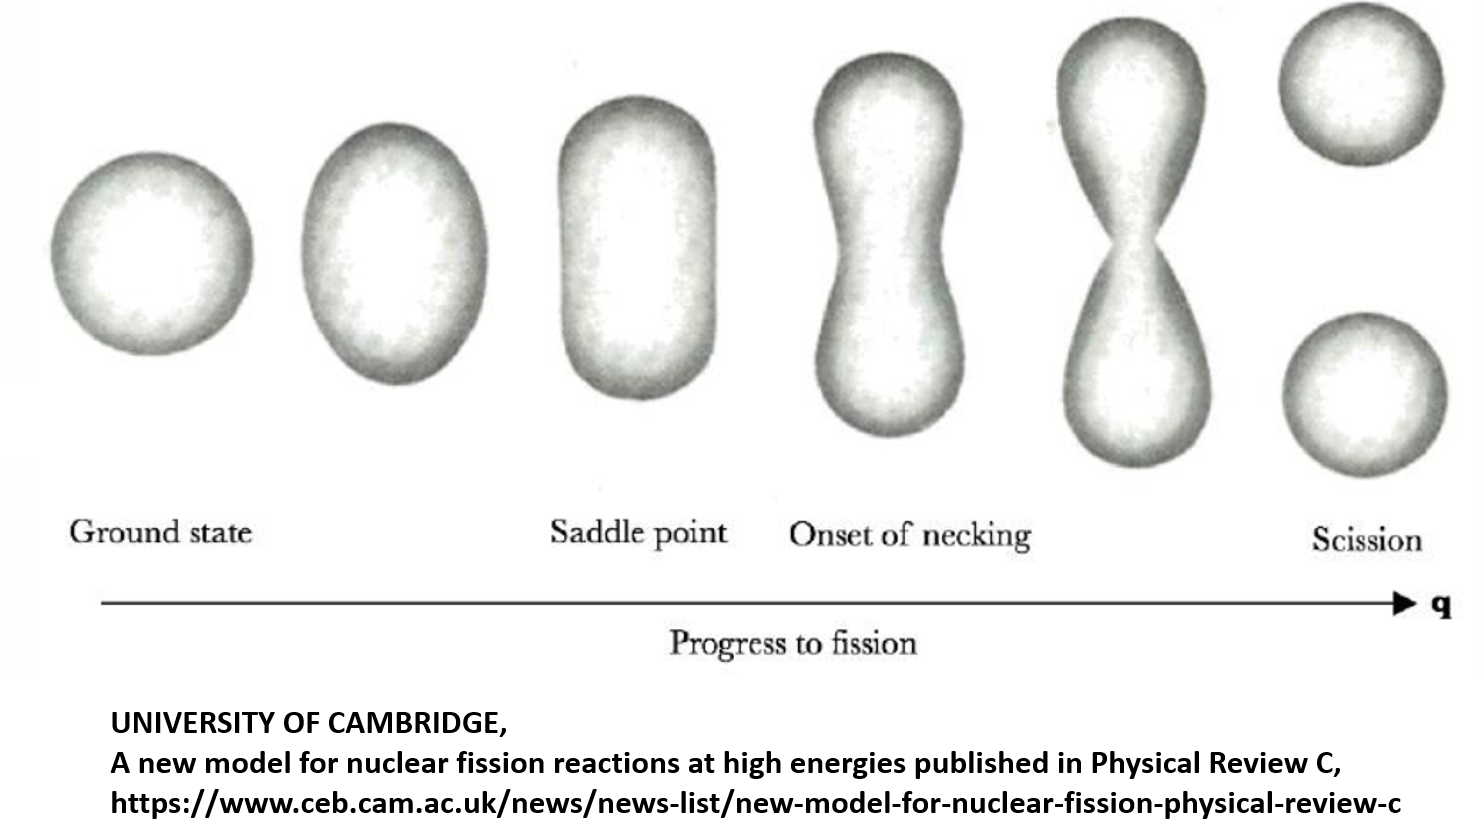
\includegraphics[scale=0.25]{fission_1.png}}
%\titlegraphic{\adjincludegraphics[height=.5\linewidth,valign=t]{heikinba.png}}

\begin{document}
\maketitle
%\frame{\tableofcontents[hideallsubsections]}




\begin{frame}{背景}
  \begin{columns}[t]
    \begin{column}{.5\textwidth}
      \begin{itemize}
        \item トンネル効果によって生じる現象が存在する
        \item 1次元模型では、ガモフによる$\alpha$崩壊の理論やWKB近似などがある
        \item 実際の核分裂は多粒子系のトンネル現象かつ複雑な形状の自由度があり、微視的な計算が困難
      \end{itemize}
    \end{column}
    \begin{column}{.5\textwidth}
      \adjincludegraphics[height=1\linewidth,valign=t]{tunneling.png}
    \end{column}
  \end{columns}
\end{frame}

\begin{frame}{論文の目的}
  J.W.Negele, Nuclear Mean-Field Theory, Physics Today 38, 24(1985)では
  \begin{itemize}
    \item 平均場理論+経路積分でトンネル効果を記述する
    \item 少数核子系(\ce{^{8}Be})の核分裂に応用する
  \end{itemize}
  ことが目的
\end{frame}

\begin{frame}{平均場理論}
  \begin{itemize}
    \item 多体系における相互作用を平均化して一体の平均ポテンシャルとして扱う手法
    \item 原子核の平均ポテンシャルは、Hartree-Fock近似によって微視的に得られる
  \end{itemize}
  \begin{columns}[t]
    \begin{column}{.5\textwidth}
      \begin{itemize}
        \item $V(r,t)$と核子の波動関数は\\自己無撞着性を持つ
        \item 核分裂のような現象が自己無撞着な集団運動として記述できる
      \end{itemize}
    \end{column}
    \begin{column}{.5\textwidth}
      \adjincludegraphics[width=1\linewidth,valign=t]{heikinba.png}
    \end{column}
  \end{columns}
\end{frame}
\begin{frame}{Hartree-Fock近似}
  \begin{itemize}
    \item Hartree-Fock(HF)近似は原子核の性質(束縛エネルギーや変形度)を上手く説明できる
    \item 時間依存のHF方程式(TDHF方程式)は核子自由度から微視的に原子核ダイナミクスを記述できる
  \end{itemize}
  \begin{block}{TDHFの問題点}
    \begin{itemize}
      \item 多体波動関数が1つのスレーター行列式で表されるという近似を用いている
            \begin{itemize}
              \item 複数のスレーター行列式の線形結合で波動関数を表すことで、より正確な状態が得られることが知られている
            \end{itemize}
      \item 核分裂反応のような多体のトンネル現象を記述できない
            \begin{itemize}
              \item 平均場が1つしかなく、核分裂していない状態と核分裂している状態の重ね合わせが記述できない
            \end{itemize}
    \end{itemize}
  \end{block}
\end{frame}



\begin{frame}{平均場理論(TDHF)で核分裂反応を記述する}
  \begin{block}{経路積分を使う理由}
    \begin{itemize}
      \item 虚時間法により、多体のトンネル現象を記述できる
      \item 鞍点法(Stationary Phase Approximation:SPA)で近似ができる
    \end{itemize}
  \end{block}
  \begin{columns}[t]
    \begin{column}{.53\textwidth}
      \vspace{-5mm}
      \begin{exampleblock}{経路積分のイメージ}
        \begin{itemize}
          \item 始状態から終状態への遷移確率振幅が経路積分で与えられる
          \item 終状態に至るまでのあらゆる経路の和を取る
          \item 作用の変分が$\delta S[q]=0$となる経路からの寄与が大きい
        \end{itemize}
      \end{exampleblock}
    \end{column}
    \begin{column}{.44\textwidth}
      \adjincludegraphics[width=1\linewidth,valign=t]{keiro.png}
    \end{column}
  \end{columns}

\end{frame}


\begin{frame}{経路積分の数式表現}
  ポテンシャルが一般化座標$q$にのみ依存する場合を考える。\\
  $K(q_f,q_i\,;t_f,t_i)$は$(q_i,t_i)$から$(q_f,t_f)$への遷移確率振幅であり、
  \begin{align*}
    K(q_f,q_i\,;t_f,t_i) & = \int\mathcal{D}q
    \exp\qty[\frac{i}{\hbar}\int_{t_i}^{t_f}dt\,\qty(\frac{m}{2}\dot{q}^2 - V(q))]                                                            \\
                         & = \int\mathcal{D}q\exp\qty[\frac{i}{\hbar}S[q]]\quad \qty(\int \mathcal{D}q \coloneqq \prod_{j=1}^{N-1} \int dq_j)
  \end{align*}
  \begin{block}{経路積分の解釈}
    $(q_i,t_i)\to(q_1,t_1)\to\cdots\to(q_{N-1},t_{N-1})\to(q_f,t_f)$
    を経たときの遷移確率振幅を考えて、中間状態に関して全ての経路の和を取ると、\\
    $\ket{q_i\,;t_i}$から$\ket{q_f\,;t_f}$への遷移確率振幅となる。
  \end{block}
\end{frame}


\begin{frame}{トンネリング解を計算する方法}
  \begin{enumerate}
    \item トンネリング解に対応するエネルギー固有値を求める
          \begin{itemize}
            \item $\trace{(E-\hat{H})^{-1}}=\sum_{n}\ev{(E-E_n)^{-1}}{E_n}$の極がエネルギー固有値
          \end{itemize}
          \begin{align*}
            \trace\frac{1}{E-\hat{H}+i\eta} & =-i\int_0^{\infty}dT\,e^{iET}\int dq\,\bra{q}e^{-i\hat{H}T}\ket{q} \\
                                            & = -i\int_0^{\infty}dT\,e^{iET}\int dq\,\int\mathcal{D}q\,e^{iS[q]}
          \end{align*}
          \begin{itemize}
            \item $q(0)=q(T)$の境界条件(周期運動)を満たした経路積分
            \item あらゆる周期解の中で、$\delta S[q(T)]=0$となるものを足し合わせる
          \end{itemize}
  \end{enumerate}
  \begin{enumerate}
    \setcounter{enumi}{1}
    \item エネルギー固有値に対応する状態(核分裂後を記述する状態)をEuler-Lagrange方程式で計算する
  \end{enumerate}
\end{frame}

\begin{frame}{エネルギー固有値を求める}
  周期$T$の運動の経路$q(T)$で、$\delta S[q(T)]=0$を満たす$q_0(T)$について$W(T)=ET+S[q_0(T)]$とする。鞍点法を用いると
  \begin{align*}
            & \int_0^{\infty}dT\,e^{iET}\underbrace{\int dq\,\int\mathcal{D}q\,e^{iS[q]}}_{\approx Ae^{iS[q_0(T)]}}
    \approx\int_0^{\infty}dT\,Ae^{i\qty(ET + S[q_0(T)])}                                                            \\
    \approx & A\sum_{m=1}^{\infty}e^{im\pi}\qty(e^{iW(T)})^m \propto \frac{e^{iW(T)}}{1+e^{iW(T)}}
  \end{align*}
  \begin{itemize}
    \item $\delta S[q_0(T)]=0$であり、$q_0(T)$はEuler-Lagrange方程式を満たす
    \item 基本周期$T$に対して、$W(mT)=mW(T)$を満たしている
    \item 周期$T$が極を与える条件$1+e^{iW(T)}=0\Leftrightarrow W(T)=(2n+1)\pi$はBohr-Sommerfeldの量子化条件に対応
  \end{itemize}
\end{frame}


\begin{frame}{1粒子系での例}
  1つの極小値を持つポテンシャル$V(q)$内を全エネルギー$E$の元で運動する1粒子について考える
  \begin{columns}[t]
    \begin{column}{.5\textwidth}
      \begin{itemize}
        \item $m\dv[2]{q_0}{t} = -\grad V(q_0)$
        \item $E-V(q)\geq0$の領域で周期$T(E)$の運動
        \item $W(T)=(2n+1)\pi$を満たす周期$T$の運動がエネルギー固有値を与える
        \item $T(E)=2\int_{q_1}^{q_2}dq\,\sqrt{\frac{m}{2(E-V(q))}}$\\から$E=E_{n}^{~0}$が求まる
      \end{itemize}
    \end{column}
    \begin{column}{.5\textwidth}
      \adjincludegraphics[width=1\linewidth,valign=t]{pot1.png}
    \end{column}
  \end{columns}
\end{frame}

\begin{frame}{1粒子系での例(図を上と同じのを使う)}
  \begin{columns}[t]
    \begin{column}{.5\textwidth}
      \begin{itemize}
        \item 先ほどは$V(q)$の極小値まわりの周期運動のみを考えていた
        \item 量子力学の結果では、トンネル効果によってポテンシャル障壁を乗り越える
        \item ポテンシャル極小値の位置$q_{\text{classical}}$は安定でない
      \end{itemize}
    \end{column}
    \begin{column}{.5\textwidth}
      \adjincludegraphics[width=1\linewidth,valign=t]{tunneling_onaji.png}
    \end{column}
  \end{columns}
\end{frame}

\begin{frame}{1粒子系での例(元のポテンシャルを点線表示、W1W2をかく)}
  $t$を純虚数として、$it\to\tau$という変換(Wick's rotation)を考えると\\
  トンネル効果が考慮できる(虚時間法)
  \begin{columns}[t]
    \begin{column}{.5\textwidth}
      \begin{itemize}
        \item $m\dv[2]{q_0}{\tau} = -\grad \qty[-V(q_0)]$
        \item 反転したポテンシャル内で$q_2\leq q\leq q_3$を運動しているように見える
        \item 虚時間で$\delta S[q_0]=0$が成立しており、鞍点法では考慮する必要がある
        \item $q_{\text{classical}}$は準安定状態であることが計算からわかる
      \end{itemize}
    \end{column}
    \begin{column}{.5\textwidth}
      \adjincludegraphics[width=1\linewidth,valign=t]{pot2.png}
    \end{column}
  \end{columns}
\end{frame}

\begin{frame}{1粒子系での例}
  虚時間方向での周期運動を考慮して$\trace(E-\hat{H})^{-1}$の計算をする\\
  $W_2(E)$は虚時間方向での$W(E)=ET+S[q_0(T)]$
  \begin{equation*}
    \trace\frac{1}{E-\hat{H}+i\eta} \propto \frac{-3e^{iW_1}-e^{-W_2}}{1+e^{iW_1}+e^{-W_2}}
  \end{equation*}
  \begin{itemize}
    \item $1+e^{iW_1(E)}=-e^{-W_2(E)}$が極となる(先ほどは$1+e^{iW_1(E_n^{~0})}=0$)
    \item $E=E_{n}^{~0}+\varDelta E_n$として、補正項$\varDelta E_n$を求めると
          \begin{equation*}
            E = E_{n}^{~0} -\frac{i\Gamma_n}{2}\,,\quad \Gamma_n = 2\frac{\omega(E_n^{~0})}{2\pi}e^{-W_2(E_n^{~0})}
          \end{equation*}
    \item $\Gamma_n$は寿命の逆数であり、準安定状態がトンネル効果で崩壊するWKB近似の式として知られている
  \end{itemize}
\end{frame}

\begin{frame}
  \frametitle{1粒子系での例}
  \begin{equation*}
    \varDelta E_n = -i\frac{\omega(E_n^{~0})}{2\pi}e^{-W_2(E_n^{~0})}\quad\text{を得る計算}
  \end{equation*}
  極を与えるエネルギーは$1+e^{iW_1(E)}=e^{-W_2(E)}$を満たしていた。\\
  また、$1+e^{iW_1(E_n^{~0})}=0$に注意すると
  \begin{align*}
     & 1+e^{iW_1(E_n^{~0}+\varDelta E_n)}=-e^{-W_2(E_n^{~0}+\varDelta E_n)}                                          \\
     & 1+\underbrace{e^{iW_1(E_n^{~0})}}_{=-1}\qty(1+i\pdv{W_1(E_n^{~0})}{E}\varDelta E_n) = -e^{-W_2(E_n^{~0})}     \\
     & \varDelta E_n = -i\frac{1}{T(E_n^{~0})}e^{-W_2(E_n^{~0})} = -i\frac{\omega(E_n^{~0})}{2\pi}e^{-W_2(E_n^{~0})}
  \end{align*}



\end{frame}

\begin{frame}{1粒子系での例(まとめ)}
  \begin{columns}[t]
    \begin{column}{.5\textwidth}
      \begin{itemize}
        \item 古典的な基底状態$q_{\text{classical}}$は\\準安定状態
        \item 虚時間に経路積分を適用するとトンネル効果が記述できる
        \item $q_3$にトンネリングした後は$q$が増大する方向へ時間発展
      \end{itemize}
    \end{column}
    \begin{column}{.5\textwidth}
      \adjincludegraphics[width=1\linewidth,valign=t]{tunneling_pot.png}
    \end{column}
  \end{columns}
  時刻$t$で$q_{\text{classical}}$の状態にいる確率$P(t)$は、$E=E_n^{~0}-i\Gamma_n/2$より
  \begin{equation*}
    P(t) = \abs{\braket{q_{\text{classical}}}{\psi(t)}}^2 = \abs{\bra{q_{\text{classical}}}e^{-iEt/\hbar}\ket{q_{\text{classical}}}}^2 = e^{-\Gamma_nt/\hbar}
  \end{equation*}
\end{frame}


\begin{frame}{核子多体系に適用する}
  \begin{columns}[t]
    \begin{column}{.5\textwidth}
      \begin{itemize}
        \item 原子核の四重極モーメント$Q$は変形度を表す
        \item $Q$に対するHFエネルギーは$Q_1$で極小値($\neq$最小値)
        \item \serifRoman{2}のポテンシャル障壁をトンネリングして\serifRoman{3}の領域へ時間発展
        \item EL方程式はHF方程式になっている
      \end{itemize}
    \end{column}
    \begin{column}{.5\textwidth}
      \adjincludegraphics[width=1\linewidth,valign=t]{kakusitataikei.png}
    \end{column}
  \end{columns}
\end{frame}


\begin{frame}{\ce{^{8}Be -> ^{4}He + ^{4}He}の計算結果(基底状態、分裂後とか+矢印の追加)}
  \adjincludegraphics[width=1\linewidth,valign=t]{Be.png}
  \begin{itemize}
    \item トンネリング後の状態は、2つの粒子に分かれた状態
    \item 本論文では、具体的な議論がなされていない
    \item Negeleの他の論文にも図は載っているが、定量的な評価は見つけられない
    \item 現在に至るまで、虚時間法の応用があまりされていない
  \end{itemize}
\end{frame}
\begin{frame}{まとめと今後の展望}
  \begin{itemize}
    \item 平均場理論+経路積分でトンネル効果を記述できる
    \item 1粒子系での例では、WKB近似の結果を再現できた
    \item 重い核(\ce{^{238}U}など)に適用するためには計算コストや精度の問題があり、工夫が必要
          \begin{itemize}
            \item 波動関数が各粒子の座標$\bm{r}_1,\,\bm{r}_2,\,\dots,\,\bm{r}_N$に依存する
            \item 多次元のポテンシャル面による透過問題(1次元ではない)
            \item 精度を上げるためには空間、時間のメッシュ数を多くする必要がある
            \item 現在のコンピュータでは計算可能
          \end{itemize}
    \item 卒研で1次元のHF計算を行い、虚時間法でトンネル現象の記述を試みる
  \end{itemize}
\end{frame}


\begin{frame}[noframenumbering]{Appendix:経路積分の数式表現}
  \begin{itemize}
    \item 時間発展演算子$U(t,t_0)=e^{-i\hat{H}(t-t_0)/\hbar}$
    \item 始状態を$\ket{\psi_i}$とすると、終状態は$\ket{\psi_f}=U(t,t_0)\ket{\psi_i}$
          \begin{equation*}
            \psi_f(q) = \int dq'\,\bra{q}U(t,t_0)\ket{q'}\bra{q'}\ket{\psi_i}
            = \int dq'\,K(q,q'\,;t,t_0)\psi_i(q')
          \end{equation*}
    \item ファインマン核$K(q_f,q_i\,;t_f,t_i)$の具体形
          \begin{equation*}
            K(q_f,q_i\,;t_f,t_i) = \int\mathcal{D}q\int\mathcal{D}p
            \exp\qty[\frac{i}{\hbar}\int_{t_i}^{t_f}dt\,(p\dot{q}-H(p,q))]
          \end{equation*}
          \begin{equation*}
            \int \mathcal{D}q \coloneqq \prod_{j=1}^{N-1} \int dq_j\;,\quad
            \int \mathcal{D}p \coloneqq \prod_{j=1}^N \int \frac{dp_j}{2\pi\hbar}\;,\quad
            t_f = t_i + N\varDelta t
          \end{equation*}
  \end{itemize}
\end{frame}

\begin{frame}[noframenumbering]{Appendixにいれたいもの}
  \begin{itemize}
    \item 経路積分の途中計算
    \item 2次元のポテンシャル面が虚時間上で極小値に落ちていく図をのせる
    \item $\trace$の計算過程
    \item $\alpha$崩壊の理論やWKB近似の理論についての説明
    \item HF方程式を載せる(一般のハミルトニアン書いて、自己む到着になることの説明)
    \item スレーター行列式とは
  \end{itemize}
\end{frame}

\end{document}